\documentclass[11pt,a4paper]{article}
\usepackage[margin=2.2cm]{geometry}
\usepackage{graphicx}
\usepackage{booktabs}
\usepackage{longtable}
\usepackage{xcolor}
\usepackage{enumitem}
\usepackage{float}
\usepackage{caption}
\usepackage[hidelinks]{hyperref}
\usepackage{url}
\setlength{\parindent}{0pt}
\setlength{\parskip}{0.55em}
\setlist{itemsep=0.15em,topsep=0.3em}
\sloppy
\newcommand{\fpath}[1]{\texttt{\detokenize{#1}}}
\newcommand{\img}[3]{%
  \begin{figure}[H]\centering
  \includegraphics[width=#3\textwidth]{images/#1}
  \caption{#2}
  \end{figure}}

\title{Website v3.1 --- Change Report\\\large Hiep Trong Space}
\author{Prepared for the owner's review and selective reversal}
\date{17 November 2026}

\begin{document}
\maketitle

\section{Summary and status}
This report lists every change made while carrying out \fpath{md/v3.1-implementation-plan.md}. Nothing has been committed or pushed: all work is uncommitted in the working tree on top of commit \fpath{f06de6b}, so every part can be reversed (see Section~\ref{sec:revert}).

\textbf{Verified.} \texttt{npm run check} (lint, typecheck, tests) passes: 77 test files, 431 tests (baseline: 75 files, 384 tests). \texttt{npm run build} passes. Browser checks ran against a production build on a \emph{copy} of the data directory; the real \fpath{data/} folder and the two protected files in \fpath{md/user/} are unchanged.

\textbf{Implemented:} global focus styling, destination zodiac loader and readiness fixes, homepage fixes, shared Task card rules, the Events dashboard (Highlights, reader, Week Calendar, editor, drafts), and the recurring School timetable.

\textbf{Not implemented:} the full Daily/Hub layout renovation shown in the approved mockups (only the card-level rules were built), several final verification passes (keyboard-only, 200\% zoom, reduced-motion in a real browser, 320\,px checks of every page), and the final screenshots set. Section~\ref{sec:open} lists these precisely.

\begin{center}
\begin{tabular}{@{}lr@{}}
\toprule
Modified tracked files & 73 \\
New files (source, tests, docs) & 27 \\
Plan phases done & 0 (baseline), 1, 2, 4, 5, part of 6 \\
\bottomrule
\end{tabular}
\end{center}

\section{Phase 1 --- Borderless focus and the Daily frame bug}
\subsection{What changed}
\begin{itemize}
\item Form controls (inputs, textareas, selects, rich-text editor, checkbox/radio/switch roles, date and time fields, search rows, toolbar buttons marked \fpath{data-focus-tint}) no longer show focus rings, outlines, border-colour changes, or focus shadows. They receive an immediate background tint instead; selected controls use a stronger tint so focus and selection differ.
\item New tokens in \fpath{src/design/tokens.css}: \fpath{--ws-focus-tint}, \fpath{--ws-focus-tint-selected}, \fpath{--cosmos-focus-tint}, \fpath{--cosmos-focus-tint-selected}. Rules live in \fpath{src/app/globals.css}.
\item Shared controls updated: \fpath{DatePickerField}, \fpath{TimeFieldControl}, \fpath{RichNoteEditor}, \fpath{SelectField}, \fpath{SegmentedControl}.
\item Per-feature CSS rules that changed a border on focus were removed from Blogs, Flashcards, Learning Room, and Tracking.
\item Static borders, invalid-state styling, and the outline on buttons and links are unchanged.
\end{itemize}

\subsection{Root cause of the large Daily frame (img35)}
\fpath{<main id="main-content" tabindex="-1">} is focusable (it is the skip-link target). After keyboard input outside the page (Win\,+\,Shift\,+\,S) and window refocus, Chrome re-matches \fpath{:focus-visible} on it and draws the global 2\,px outline around the whole content area. Reproduced on the old build (computed outline \texttt{solid 2px}); on v3.1 the same state computes \texttt{none}. Non-interactive focus targets with \fpath{tabindex="-1"} now keep focus but draw no frame.

\begin{figure}[H]\centering
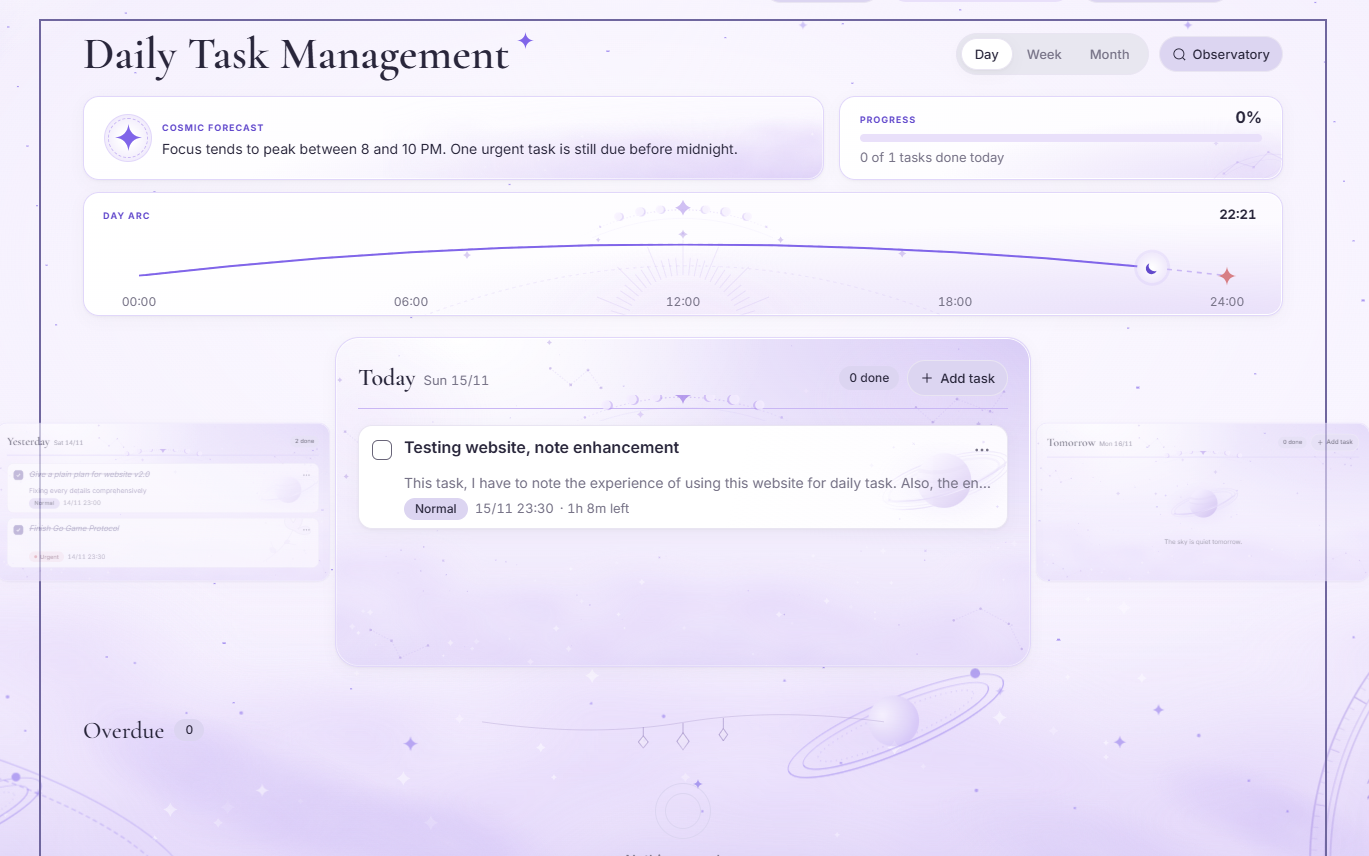
\includegraphics[width=0.48\textwidth]{images/img35-original.png}\hfill
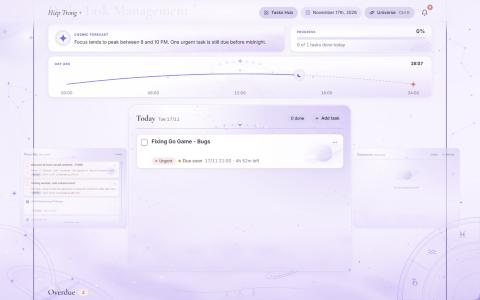
\includegraphics[width=0.48\textwidth]{images/focus-frame-before.jpg}
\caption{Left: the reported frame (your screenshot img35). Right: the old build reproducing the frame on the focused page container.}
\end{figure}

\subsection{Task brief-card alignment (shared rules)}
New \fpath{src/features/tasks/task-brief.module.css} plus tokens \fpath{--brief-*}. The checkbox, title and menu now share one grid header row; measured in the browser, all three sit on the same vertical centre. Descriptions use one two-line clamp in Daily and Hub (ellipsis on line two, long unbroken text wraps), and the reserved height is derived from the text's own line height. The Daily card height is now computed instead of fixed at 104/132\,px.

\img{daily-after.jpg}{Daily page on the v3.1 production build (cards use the shared header row and two-line description slot).}{0.85}

\section{Phase 2 --- Zodiac loading transition and homepage}
\subsection{Loader replaces Cosmic Launch}
\begin{itemize}
\item \fpath{CosmicLaunchOverlay.tsx} and its test were removed. New: \fpath{ZodiacLoaderOverlay.tsx}, \fpath{zodiac-loader.module.css}, \fpath{route-zodiac.ts}; \fpath{TransitionProvider.tsx} was rewritten.
\item Navigation starts immediately. Daily and Tasks Hub show Aries, Events shows Taurus, other mapped features keep their registry sign, and Home and unmapped routes show a plain spinner.
\item No minimum display time and no waiting for the drawing: the overlay ends when the destination pathname is reached \emph{and} the destination signals readiness. A 10\,s failsafe remains. Reduced motion shows a static symbol with loading text. Back/Forward keeps a light fade. Same-path query or hash changes show no loader.
\item Readiness is tracked per navigation, so stale signals cannot complete a later visit.
\item Eleven feature pages (Achievements, AI Engineering, APCS, Blogs, Entertainment, Events, Flashcards, Learning Room, Milestones, Projects, Tracking) used to signal ``ready'' on page mount, before data loaded. Each view now signals after its primary query finishes.
\item \fpath{ZodiacIllumination} gained a \fpath{presentation} prop (\texttt{hover}, \texttt{static}, \texttt{loader}).
\end{itemize}

\subsection{Measured navigation time}
Headless Chromium, production builds, copied data. Three cold samples (cache cleared) and five warm samples per route; values are median (min--max) in milliseconds. ``Released'' is when the loader reports the page ready; ``overlay gone'' is when it has fully disappeared.

\begin{center}
\small
\begin{tabular}{@{}llrrrr@{}}
\toprule
Route & Run & Old released & Old gone & v3.1 released & v3.1 gone \\
\midrule
Daily $\to$ Hub & cold & 2309 & 3011 & 45 & 195 \\
Daily $\to$ Hub & warm & 2309 & 3009 & 22 & 177 \\
Hub $\to$ Daily & cold & 2309 & 3013 & 98 & 251 \\
Hub $\to$ Daily & warm & 2308 & 3010 & 38 & 193 \\
Daily $\to$ Home & cold & 2312 & 3011 & 157 & 213 \\
Daily $\to$ Home & warm & 2311 & 3016 & 39 & 177 \\
Home $\to$ Events & cold & 2308 & 3011 & 213 & 365 \\
Home $\to$ Events & warm & 2309 & 3011 & 48 & 198 \\
\bottomrule
\end{tabular}
\end{center}
First editor open, save, edit and delete of an event were already fast on the old build (medians 14--36\,ms) and are unchanged in practice on v3.1 (14--43\,ms), so no extra performance change was made there.

\subsection{Homepage}
\begin{itemize}
\item Homepage presentation text can no longer be selected; inputs, dialogs and overlays keep normal selection.
\item The collection heading and the first card now share one left edge: the gallery inset is measured from the heading's content box. Measured: 0\,px difference at 1440 and 1920\,px widths. The last card stays reachable.
\item Zodiac cards are fully drawn at rest; hover or keyboard focus only raises a gentle glow (no drawing, scaling, lifting or moving light).
\end{itemize}

\section{Phases 4 and 5 --- Events dashboard and School timetable}
\subsection{Data model (backward compatible)}
\begin{itemize}
\item \fpath{src/contracts/event.ts}: new category \texttt{contest}; \texttt{school} kept as a read-only legacy value; event \texttt{kind} (\texttt{event} or \texttt{class}); \texttt{highlighted}, \texttt{status}, \texttt{revision}; class schedule with default revisions, weekly overrides, end limit, cancel and delete cutoffs; unknown legacy fields pass through.
\item New pure domain modules \fpath{src/domain/event-occurrence.ts} (week keys, effective defaults, occurrence resolution, scoped edit/cancel/delete, conflict detection over the whole future, expiry, highlights, counts) and \fpath{src/domain/event-editor-values.ts} (editor values and minimal patches).
\item Storage: \fpath{JsonFileStore} gained a locked \texttt{transaction} method and a one-time timestamped backup with a count-only summary before the first format-changing write. The backup was verified byte-identical to the original \fpath{events.json}.
\item \fpath{EventService} rewritten: normalise-on-read (no write on listing), revision checks, class creation with conflict blocking, scoped occurrence mutations, explicit Convert to class, and refusal to delete a recurring class without a scope.
\end{itemize}

\subsection{API and client}
New \fpath{GET /api/events/occurrences?from=\&to=} (half-open Asia/Saigon date range, at most 366 days) and \fpath{POST /api/events/[id]/occurrences} (edit, cancel or delete; this week or onward). Client queries load occurrences in 12-week chunks. Drafts now carry kind, end time, highlight, source revision, and a class occurrence and scope, so two weeks of one series never overwrite each other. Old drafts that lack end fields no longer erase a stored end time (a bug found and fixed).

\subsection{Interface}
\begin{itemize}
\item Heading ``Events \& schedule''; counters say ``upcoming exams (next 7 days)'' and name the displayed horizon.
\item Highlights: opt-in, nearest three, Show all / Show less with a bounded scroll area.
\item Upcoming and Past load in 12-week batches (Load more / Load older). Events expire at their end time (or start time when there is no end); ongoing events are labelled.
\item Editor: category required (Exam, Meeting, Deadline, Contest; no School for new events), optional end date and time, one ``Location or link'' field, ``Highlight this event'' replacing the online and exam checkboxes. Legacy School events show a ``Convert to class'' action.
\item Detail pane: six-line notes preview with ``See more'' only when the text overflows, opening a centered full reader (75\% width, capped at 1140\,px; full-screen on phones).
\item Week Calendar moved out of the tabs into its own panel (80\% width, capped at 1440\,px) with Overview, day agenda and whole-week modes.
\item School timetable: seven days by four periods, afternoon divider, canceled classes struck through with a replacement option, add-class from an empty cell, horizontal scroll with a sticky time column on narrow screens.
\item Event title weights raised (main title 600, titles 500).
\end{itemize}

\img{events-dashboard.jpg}{Events \& schedule dashboard (copied data).}{0.85}
\img{events-detail-preview.jpg}{Detail pane with the six-line preview and ``See more''.}{0.85}
\img{events-reader.jpg}{Full event reader.}{0.85}
\img{week-calendar.jpg}{Week Calendar panel in Overview mode.}{0.85}
\img{timetable.jpg}{School timetable for the current week.}{0.85}
\img{class-editor.jpg}{New class editor opened from an empty timetable cell, prefilled with date and period.}{0.85}

\begin{figure}[H]\centering
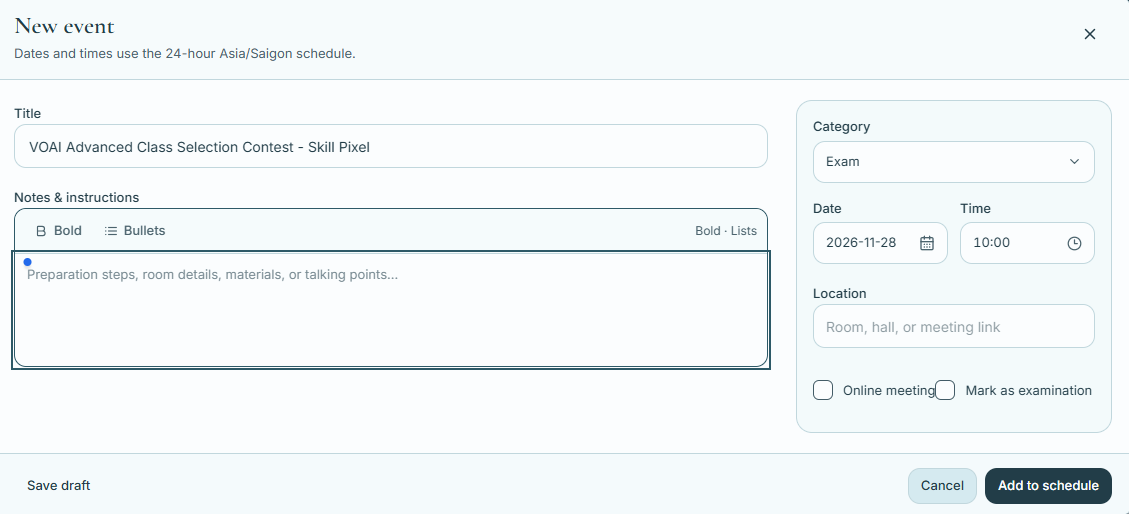
\includegraphics[width=0.48\textwidth]{images/img41-original.png}\hfill
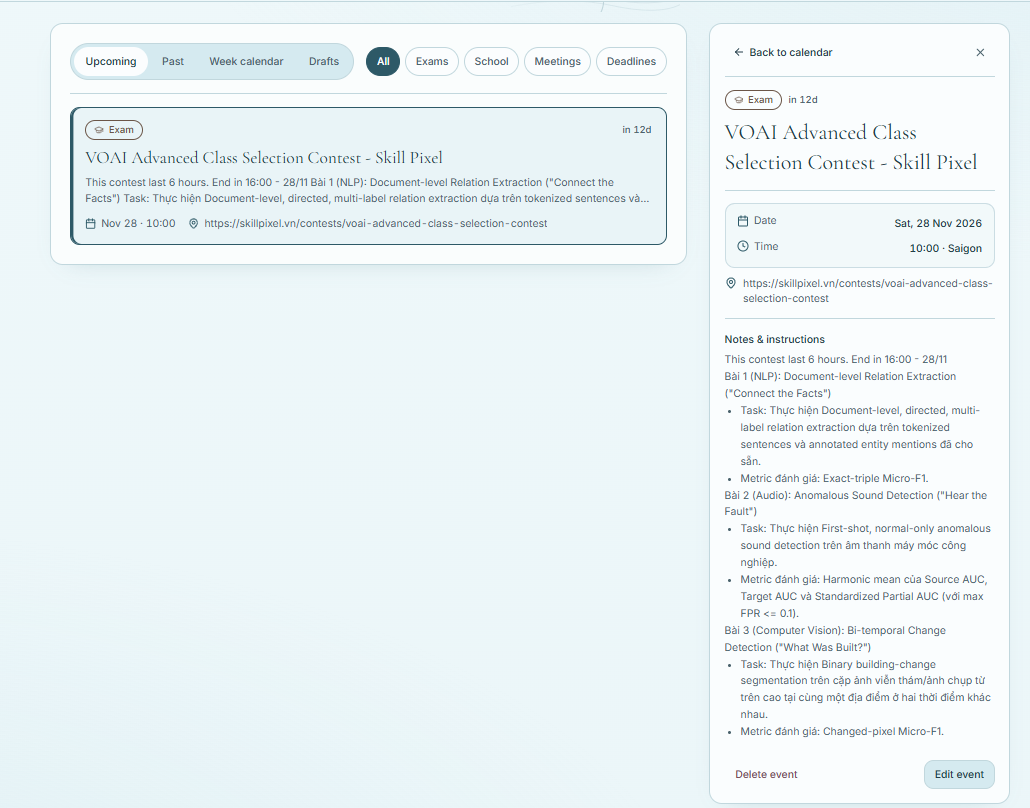
\includegraphics[width=0.48\textwidth]{images/img42-original.png}
\caption{Your original reference screenshots for the Event editor (left) and detail preview (right), for before/after comparison.}
\end{figure}

\subsection{Rules covered by tests}
The dated example from plan Section~7.3 (weeks of 16 Nov to 14 Dec), same-cell and future-only conflicts, conflicts beyond 12 weeks, canceled slots, scoped cancel and delete, moved-date occurrences, expiry boundaries, highlight ordering, and legacy record preservation are covered by 21 domain tests, 11 service tests, and 8 dashboard interface tests.

\section{Phase 6 --- Task renovation (partial)}
Mockups were published as a private design canvas (7 boards: Daily day, phone, week and month; Hub desktop and phone; card states; form and detail). You approved them without notes. Implemented from them so far: the shared card rules above, and Hub note cards now size to their content (the fixed 240\,px body was removed; cards without a description no longer reserve empty space). The wider layout changes in the mockups were \textbf{not} built.

\section{Documentation changes}
\begin{itemize}
\item \fpath{md/agents/shared/uiux.md}: new focus rule, destination zodiac loader section, Cosmic Launch marked historical.
\item \fpath{md/agents/homepage/readme.md}: Section 3.4 (selection, shared gutter, static zodiac cards).
\item \fpath{md/agents/tasks/readme.md}: Section 3.3 (card anatomy); \fpath{md/agents/tasks/reports.md}: dated entry.
\item Originals archived with matching hashes under \fpath{md/archive/v3.1-pre-update/}.
\item New \fpath{md/v3.1-suggestions.md}: 4 covered findings and 7 proposals awaiting your decision.
\end{itemize}

\section{Tests changed}
\begin{itemize}
\item Removed: \fpath{cosmic-launch.test.tsx} (replaced by \fpath{route-loader.test.tsx}) and \fpath{event-editing.test.tsx} (replaced by \fpath{events-dashboard.test.tsx}); their behaviour was superseded by the plan.
\item Updated: gallery geometry expectations, the zodiac hover test (now asserts static-at-rest), the Hub fixed-height assertion, event editor and draft service tests.
\item Added: occurrence domain, event service, route loader, and Events dashboard tests.
\end{itemize}

\section{Known gaps and honest caveats}\label{sec:open}
\begin{itemize}
\item The Daily/Hub layout renovation beyond card rules is not built.
\item Not verified in a real browser: keyboard-only walkthrough of every control, 200\% zoom, reduced motion, and 320\,px for every page (the Events dashboard, timetable and Week Calendar at 320\,px were checked: no page-level horizontal overflow). Task carousel 3.5-card measurement was not re-measured after the card-height change.
\item Weekly classes create no reminders (class series are excluded from notification sources).
\item Deleting an ordinary event has no confirmation (pre-existing behaviour).
\item The Events preview page (\fpath{/preview/events-pilot}) still shows the older editor.
\item A page reload could briefly show Events skeletons while the clock syncs; this is intentional.
\end{itemize}

\section{How to reverse parts}\label{sec:revert}
Nothing is committed. To reverse a tracked file: \texttt{git checkout -- <file>}. To remove a new file: delete it. Reverse whole areas together, otherwise imports break:
\begin{description}
\item[Focus styling] \fpath{src/app/globals.css}, \fpath{src/design/tokens.css} (focus tokens), the five shared controls, and the four feature CSS modules.
\item[Zodiac loader] restore \fpath{CosmicLaunchOverlay.tsx} with \texttt{git checkout}, revert \fpath{TransitionProvider.tsx} and \fpath{transition-rules.ts}, delete the three new loader files, restore the old transition test, and revert the 11 view files and page files (readiness).
\item[Homepage] \fpath{HorizontalGallery.tsx}, \fpath{FeatureCard.tsx}, \fpath{FeatureThumbnail.tsx}, \fpath{feature-collection.module.css}, \fpath{home-journey.module.css}, and the matching test.
\item[Task card rules] \fpath{TaskCard.tsx}, \fpath{TaskMenu.tsx}, \fpath{task-note.module.css}, \fpath{daily-task-card.module.css}, \fpath{day-task-list.module.css}, delete \fpath{task-brief.module.css}.
\item[Events and timetable] the largest area: contracts, domain, services, storage, API routes, client queries, everything in \fpath{src/features/events/}, and the Events tests. Revert it together; the stored data format is backward compatible, and a pre-v3.1 backup is written next to \fpath{events.json} on the first write.
\end{description}
If any new-format events were saved with v3.1, restore the matching \fpath{events.json.pre-v3.1-*.bak} together with the old code before reopening data with older code.

\appendix
\section{Modified files (line counts from git)}
\begin{longtable}{p{0.72\textwidth}rr}
\toprule File & Added & Removed \\
\midrule\endhead
\texttt{md/\allowbreak{}agents/\allowbreak{}homepage/\allowbreak{}readme.md} & 6 & 0 \\
\texttt{md/\allowbreak{}agents/\allowbreak{}shared/\allowbreak{}uiux.md} & 14 & 2 \\
\texttt{md/\allowbreak{}agents/\allowbreak{}tasks/\allowbreak{}readme.md} & 7 & 0 \\
\texttt{md/\allowbreak{}agents/\allowbreak{}tasks/\allowbreak{}reports.md} & 5 & 0 \\
\texttt{src/\allowbreak{}app/\allowbreak{}(workspace)/\allowbreak{}achievements/\allowbreak{}page.tsx} & 1 & 2 \\
\texttt{src/\allowbreak{}app/\allowbreak{}(workspace)/\allowbreak{}ai-engineering/\allowbreak{}page.tsx} & 1 & 2 \\
\texttt{src/\allowbreak{}app/\allowbreak{}(workspace)/\allowbreak{}apcs/\allowbreak{}page.tsx} & 1 & 2 \\
\texttt{src/\allowbreak{}app/\allowbreak{}(workspace)/\allowbreak{}blogs/\allowbreak{}page.tsx} & 1 & 2 \\
\texttt{src/\allowbreak{}app/\allowbreak{}(workspace)/\allowbreak{}entertainment/\allowbreak{}page.tsx} & 1 & 2 \\
\texttt{src/\allowbreak{}app/\allowbreak{}(workspace)/\allowbreak{}events/\allowbreak{}page.tsx} & 1 & 2 \\
\texttt{src/\allowbreak{}app/\allowbreak{}(workspace)/\allowbreak{}flashcards/\allowbreak{}page.tsx} & 1 & 2 \\
\texttt{src/\allowbreak{}app/\allowbreak{}(workspace)/\allowbreak{}learning-room/\allowbreak{}page.tsx} & 1 & 2 \\
\texttt{src/\allowbreak{}app/\allowbreak{}(workspace)/\allowbreak{}milestones/\allowbreak{}page.tsx} & 1 & 2 \\
\texttt{src/\allowbreak{}app/\allowbreak{}(workspace)/\allowbreak{}projects/\allowbreak{}page.tsx} & 1 & 2 \\
\texttt{src/\allowbreak{}app/\allowbreak{}(workspace)/\allowbreak{}tracking/\allowbreak{}page.tsx} & 1 & 2 \\
\texttt{src/\allowbreak{}app/\allowbreak{}api/\allowbreak{}events/\allowbreak{}route.ts} & 2 & 1 \\
\texttt{src/\allowbreak{}app/\allowbreak{}globals.css} & 120 & 69 \\
\texttt{src/\allowbreak{}client/\allowbreak{}queries/\allowbreak{}events.ts} & 136 & 17 \\
\texttt{src/\allowbreak{}contracts/\allowbreak{}event-draft.ts} & 53 & 5 \\
\texttt{src/\allowbreak{}contracts/\allowbreak{}event.ts} & 210 & 18 \\
\texttt{src/\allowbreak{}design/\allowbreak{}tokens.css} & 12 & 0 \\
\texttt{src/\allowbreak{}domain/\allowbreak{}event-domain.ts} & 13 & 0 \\
\texttt{src/\allowbreak{}features/\allowbreak{}achievements/\allowbreak{}AchievementsView.tsx} & 2 & 0 \\
\texttt{src/\allowbreak{}features/\allowbreak{}ai-engineering/\allowbreak{}AiEngineeringView.tsx} & 2 & 0 \\
\texttt{src/\allowbreak{}features/\allowbreak{}apcs/\allowbreak{}ApcsView.tsx} & 2 & 0 \\
\texttt{src/\allowbreak{}features/\allowbreak{}blogs/\allowbreak{}WritingRoomView.tsx} & 2 & 0 \\
\texttt{src/\allowbreak{}features/\allowbreak{}blogs/\allowbreak{}writing-room.module.css} & 0 & 10 \\
\texttt{src/\allowbreak{}features/\allowbreak{}entertainment/\allowbreak{}EntertainmentView.tsx} & 3 & 4 \\
\texttt{src/\allowbreak{}features/\allowbreak{}events/\allowbreak{}EventsView.tsx} & 999 & 1570 \\
\texttt{src/\allowbreak{}features/\allowbreak{}events/\allowbreak{}event-editor.ts} & 19 & 43 \\
\texttt{src/\allowbreak{}features/\allowbreak{}events/\allowbreak{}events.module.css} & 28 & 2 \\
\texttt{src/\allowbreak{}features/\allowbreak{}events/\allowbreak{}pilot/\allowbreak{}EventsPilotPrototype.tsx} & 13 & 17 \\
\texttt{src/\allowbreak{}features/\allowbreak{}events/\allowbreak{}pilot/\allowbreak{}events-pilot-fixtures.ts} & 24 & 6 \\
\texttt{src/\allowbreak{}features/\allowbreak{}flashcards/\allowbreak{}FlashcardsView.tsx} & 2 & 0 \\
\texttt{src/\allowbreak{}features/\allowbreak{}flashcards/\allowbreak{}flashcards.module.css} & 0 & 6 \\
\texttt{src/\allowbreak{}features/\allowbreak{}home/\allowbreak{}feature-collection/\allowbreak{}FeatureCard.tsx} & 1 & 60 \\
\texttt{src/\allowbreak{}features/\allowbreak{}home/\allowbreak{}feature-collection/\allowbreak{}FeatureThumbnail.tsx} & 7 & 1 \\
\texttt{src/\allowbreak{}features/\allowbreak{}home/\allowbreak{}feature-collection/\allowbreak{}HorizontalGallery.tsx} & 13 & 5 \\
\texttt{src/\allowbreak{}features/\allowbreak{}home/\allowbreak{}feature-collection/\allowbreak{}feature-collection.module.css} & 30 & 0 \\
\texttt{src/\allowbreak{}features/\allowbreak{}home/\allowbreak{}home-journey.module.css} & 22 & 1 \\
\texttt{src/\allowbreak{}features/\allowbreak{}learning-room/\allowbreak{}LearningRoomView.tsx} & 2 & 0 \\
\texttt{src/\allowbreak{}features/\allowbreak{}learning-room/\allowbreak{}learning-room.module.css} & 0 & 8 \\
\texttt{src/\allowbreak{}features/\allowbreak{}milestones/\allowbreak{}MilestonesView.tsx} & 2 & 0 \\
\texttt{src/\allowbreak{}features/\allowbreak{}projects/\allowbreak{}ProjectsView.tsx} & 2 & 0 \\
\texttt{src/\allowbreak{}features/\allowbreak{}tasks/\allowbreak{}TaskCard.tsx} & 61 & 73 \\
\texttt{src/\allowbreak{}features/\allowbreak{}tasks/\allowbreak{}TaskMenu.tsx} & 1 & 1 \\
\texttt{src/\allowbreak{}features/\allowbreak{}tasks/\allowbreak{}daily-task-card.module.css} & 4 & 5 \\
\texttt{src/\allowbreak{}features/\allowbreak{}tasks/\allowbreak{}day-task-list.module.css} & 8 & 2 \\
\texttt{src/\allowbreak{}features/\allowbreak{}tasks/\allowbreak{}task-note.module.css} & 1 & 9 \\
\texttt{src/\allowbreak{}features/\allowbreak{}tracking/\allowbreak{}TrackingView.tsx} & 2 & 0 \\
\texttt{src/\allowbreak{}features/\allowbreak{}tracking/\allowbreak{}tracking.module.css} & 0 & 5 \\
\texttt{src/\allowbreak{}features/\allowbreak{}transitions/\allowbreak{}CosmicLaunchOverlay.tsx} & 0 & 320 \\
\texttt{src/\allowbreak{}features/\allowbreak{}transitions/\allowbreak{}TransitionProvider.tsx} & 111 & 160 \\
\texttt{src/\allowbreak{}features/\allowbreak{}transitions/\allowbreak{}transition-rules.ts} & 6 & 3 \\
\texttt{src/\allowbreak{}features/\allowbreak{}zodiac/\allowbreak{}ZodiacIllumination.tsx} & 20 & 3 \\
\texttt{src/\allowbreak{}features/\allowbreak{}zodiac/\allowbreak{}types.ts} & 6 & 0 \\
\texttt{src/\allowbreak{}features/\allowbreak{}zodiac/\allowbreak{}zodiac-illumination.module.css} & 8 & 1 \\
\texttt{src/\allowbreak{}services/\allowbreak{}event-draft-service.ts} & 201 & 109 \\
\texttt{src/\allowbreak{}services/\allowbreak{}event-service.ts} & 352 & 20 \\
\texttt{src/\allowbreak{}services/\allowbreak{}storage/\allowbreak{}json-store.ts} & 70 & 3 \\
\texttt{src/\allowbreak{}services/\allowbreak{}timed-sources.ts} & 5 & 1 \\
\texttt{src/\allowbreak{}ui/\allowbreak{}DatePickerField.tsx} & 8 & 7 \\
\texttt{src/\allowbreak{}ui/\allowbreak{}RichNoteEditor.tsx} & 5 & 4 \\
\texttt{src/\allowbreak{}ui/\allowbreak{}SegmentedControl.tsx} & 1 & 0 \\
\texttt{src/\allowbreak{}ui/\allowbreak{}SelectField.tsx} & 1 & 1 \\
\texttt{src/\allowbreak{}ui/\allowbreak{}TimeFieldControl.tsx} & 7 & 7 \\
\texttt{tests/\allowbreak{}features/\allowbreak{}events/\allowbreak{}event-editing.test.tsx} & 0 & 722 \\
\texttt{tests/\allowbreak{}features/\allowbreak{}events/\allowbreak{}event-editor.test.ts} & 80 & 33 \\
\texttt{tests/\allowbreak{}features/\allowbreak{}home/\allowbreak{}feature-collection.test.tsx} & 14 & 13 \\
\texttt{tests/\allowbreak{}features/\allowbreak{}tasks/\allowbreak{}task-inspector-and-daily-polish.test.tsx} & 3 & 2 \\
\texttt{tests/\allowbreak{}features/\allowbreak{}transitions/\allowbreak{}cosmic-launch.test.tsx} & 0 & 229 \\
\texttt{tests/\allowbreak{}services/\allowbreak{}event-draft-service.test.ts} & 4 & 3 \\
\texttt{tests/\allowbreak{}zodiac-component.test.tsx} & 8 & 54 \\
\bottomrule
\end{longtable}


\section{New files}
\begin{longtable}{p{0.95\textwidth}}
\toprule New file \\
\midrule\endhead
\texttt{md/\allowbreak{}archive/\allowbreak{}v3.1-pre-update/\allowbreak{}agents/\allowbreak{}homepage/\allowbreak{}readme.md} \\
\texttt{md/\allowbreak{}archive/\allowbreak{}v3.1-pre-update/\allowbreak{}agents/\allowbreak{}shared/\allowbreak{}uiux.md} \\
\texttt{md/\allowbreak{}archive/\allowbreak{}v3.1-pre-update/\allowbreak{}agents/\allowbreak{}tasks/\allowbreak{}readme.md} \\
\texttt{md/\allowbreak{}v3.1-implementation-plan.md} \\
\texttt{md/\allowbreak{}v3.1-suggestions.md} \\
\texttt{src/\allowbreak{}app/\allowbreak{}api/\allowbreak{}events/\allowbreak{}[id]/\allowbreak{}occurrences/\allowbreak{}route.ts} \\
\texttt{src/\allowbreak{}app/\allowbreak{}api/\allowbreak{}events/\allowbreak{}occurrences/\allowbreak{}route.ts} \\
\texttt{src/\allowbreak{}domain/\allowbreak{}event-editor-values.ts} \\
\texttt{src/\allowbreak{}domain/\allowbreak{}event-occurrence.ts} \\
\texttt{src/\allowbreak{}features/\allowbreak{}events/\allowbreak{}EventBadges.tsx} \\
\texttt{src/\allowbreak{}features/\allowbreak{}events/\allowbreak{}EventDetailPane.tsx} \\
\texttt{src/\allowbreak{}features/\allowbreak{}events/\allowbreak{}EventEditorDialog.tsx} \\
\texttt{src/\allowbreak{}features/\allowbreak{}events/\allowbreak{}EventReader.tsx} \\
\texttt{src/\allowbreak{}features/\allowbreak{}events/\allowbreak{}EventsModal.tsx} \\
\texttt{src/\allowbreak{}features/\allowbreak{}events/\allowbreak{}HighlightsSection.tsx} \\
\texttt{src/\allowbreak{}features/\allowbreak{}events/\allowbreak{}SchoolTimetable.tsx} \\
\texttt{src/\allowbreak{}features/\allowbreak{}events/\allowbreak{}WeekCalendarPanel.tsx} \\
\texttt{src/\allowbreak{}features/\allowbreak{}events/\allowbreak{}events-format.ts} \\
\texttt{src/\allowbreak{}features/\allowbreak{}events/\allowbreak{}events-overlays.module.css} \\
\texttt{src/\allowbreak{}features/\allowbreak{}tasks/\allowbreak{}task-brief.module.css} \\
\texttt{src/\allowbreak{}features/\allowbreak{}transitions/\allowbreak{}ZodiacLoaderOverlay.tsx} \\
\texttt{src/\allowbreak{}features/\allowbreak{}transitions/\allowbreak{}route-zodiac.ts} \\
\texttt{src/\allowbreak{}features/\allowbreak{}transitions/\allowbreak{}zodiac-loader.module.css} \\
\texttt{tests/\allowbreak{}domain/\allowbreak{}event-occurrence.test.ts} \\
\texttt{tests/\allowbreak{}features/\allowbreak{}events/\allowbreak{}events-dashboard.test.tsx} \\
\texttt{tests/\allowbreak{}features/\allowbreak{}transitions/\allowbreak{}route-loader.test.tsx} \\
\texttt{tests/\allowbreak{}services/\allowbreak{}event-service.test.ts} \\
\bottomrule
\end{longtable}

\end{document}
